% THIS IS SIGPROC-SP.TEX - VERSION 3.1
% WORKS WITH V3.2SP OF ACM_PROC_ARTICLE-SP.CLS
% APRIL 2009
%
% It is an example file showing how to use the 'acm_proc_article-sp.cls' V3.2SP
% LaTeX2e document class file for Conference Proceedings submissions.
% ----------------------------------------------------------------------------------------------------------------
% This .tex file (and associated .cls V3.2SP) *DOES NOT* produce:
%       1) The Permission Statement
%       2) The Conference (location) Info information
%       3) The Copyright Line with ACM data
%       4) Page numbering
% ---------------------------------------------------------------------------------------------------------------
% It is an example which *does* use the .bib file (from which the .bbl file
% is produced).
% REMEMBER HOWEVER: After having produced the .bbl file,
% and prior to final submission,
% you need to 'insert'  your .bbl file into your source .tex file so as to provide
% ONE 'self-contained' source file.
%
% Questions regarding SIGS should be sent to
% Adrienne Griscti ---> griscti@acm.org
%
% Questions/suggestions regarding the guidelines, .tex and .cls files, etc. to
% Gerald Murray ---> murray@hq.acm.org
%
% For tracking purposes - this is V3.1SP - APRIL 2009

\documentclass{acm_proc_article-sp}
\usepackage{float}

\begin{document}

\title{Analysis \& Comparison of Scheduling Algorithm Performance using the Java Programming Language}
%\subtitle{[Extended Abstract]}
%
% You need the command \numberofauthors to handle the 'placement
% and alignment' of the authors beneath the title.
%
% For aesthetic reasons, we recommend 'three authors at a time'
% i.e. three 'name/affiliation blocks' be placed beneath the title.
%
% NOTE: You are NOT restricted in how many 'rows' of
% "name/affiliations" may appear. We just ask that you restrict
% the number of 'columns' to three.
%
% Because of the available 'opening page real-estate'
% we ask you to refrain from putting more than six authors
% (two rows with three columns) beneath the article title.
% More than six makes the first-page appear very cluttered indeed.
%
% Use the \alignauthor commands to handle the names
% and affiliations for an 'aesthetic maximum' of six authors.
% Add names, affiliations, addresses for
% the seventh etc. author(s) as the argument for the
% \additionalauthors command.
% These 'additional authors' will be output/set for you
% without further effort on your part as the last section in
% the body of your article BEFORE References or any Appendices.

\numberofauthors{1} %  in this sample file, there are a *total*
% of EIGHT authors. SIX appear on the 'first-page' (for formatting
% reasons) and the remaining two appear in the \additionalauthors section.
%
\author{
% You can go ahead and credit any number of authors here,
% e.g. one 'row of three' or two rows (consisting of one row of three
% and a second row of one, two or three).
%
% The command \alignauthor (no curly braces needed) should
% precede each author name, affiliation/snail-mail address and
% e-mail address. Additionally, tag each line of
% affiliation/address with \affaddr, and tag the
% e-mail address with \email.
%
% 1st. author
\alignauthor
Connor Goddard\\%\titlenote{Connor Goddard (clg11)}\\
       \affaddr{Computer Science}\\
       \affaddr{Aberystwyth University, Aberystwyth}\\
       \vspace{2mm}
       \email{clg11@aber.ac.uk}
}
% There's nothing stopping you putting the seventh, eighth, etc.
% author on the opening page (as the 'third row') but we ask,
% for aesthetic reasons that you place these 'additional authors'
% in the \additional authors block, viz.

%\additionalauthors{Additional authors: John Smith (The Th{\o}rv{\"a}ld Group,
%email: {\texttt{jsmith@affiliation.org}}) and Julius P.~Kumquat
%(The Kumquat Consortium, email: {\texttt{jpkumquat@consortium.net}}).}
%\date{30 July 1999}

% Just remember to make sure that the TOTAL number of authors
% is the number that will appear on the first page PLUS the
% number that will appear in the \additionalauthors section.

\maketitle
\begin{abstract}
Process scheduling algorithms form a core part of modern computer systems nowadays, by enabling the ``illusion" of multi-tasking to take place within operating systems. Choosing a suitable algorithm can be crucial to the efficiency and underlying speed of a system. The purpose of this investigation is to compare and contrast a selection of process scheduling algorithms to determine the differences in performance when presented with various collections of jobs. These algorithms will be implemented into an existing simulator written in the Java programming language, and tested using a variety of different processes and priorities. 

Through extensive experimental testing, it was discovered that the use of preemptive scheduling algorithms can lead to a greater level of throughput, while minimising latency. In addition, non-deterministic algorithms can provide better performance for jobs that require a high level of I/O operations that in turn cause the halting of such jobs on the CPU. 

\end{abstract}

%A category including the fourth, optional field follows...
\category{F.2.2}{Analysis of Algorithms and Problem Complexity}{Nonnumerical Algorithms and Problems}[Sequencing and Scheduling]

\keywords{Scheduling, job queue, algorithms, processes, simulator} % NOT required for Proceedings

\section{Introduction}
Scheduling algorithms play a vital role in computing today. Their purpose is to allocate system resources (e.g. processor time, memory space) to a collection of waiting processes in an attempt to aid in the `load balancing' of a system.

Often the choice of algorithm will depend on the prioritisation of three key factors; \textbf{throughput}, \textbf{latency} and \textbf{fairness}. Throughput details the total number of processes that are completed within a given duration of time, latency is the amount of time taken to allocate resources to a given process, and fairness determines the amount of resources (e.g. CPU time) given to a process (generally determined by the priority of the process).

\subsection{Aims \& Objectives}  

This investigation intends to analyse, compare and contrast a selection of scheduling algorithms to determine:
\vspace{-3mm}

\begin{enumerate}

\item Whether there is a link between the use of preemptive scheduling algorithms and the time taken to complete the first job.  

\item If the use of a non-deterministic scheduling algorithm over deterministic affects the mean time to finish a job. 

\item If any scheduling algorithms significantly increase or decrease the overall processing time for a typical collection of jobs.

\end{enumerate}

\subsection{Hypothesis}

As part of the investigation, it is predicted that the results will give support to a number of hypotheses:
\vspace{-3mm}

\begin{enumerate}

\item The use of certain preemptive algorithms will result in the completion time for the first job to be consistently smaller than that of other algorithms. 

\textit{This is due to preemptive algorithms having the ability to prioritise the job they select based on set criteria, which is the case of this investigation is the job with the shortest remaining execution time.}

\item Select deterministic preemptive algorithms will on average complete a single job faster than a non-preemptive deterministic algorithm.

\textit{As the preemptive algorithm selected for this investigation prioritises jobs by remaining execution length, on average the chance of an executing job being halted by a new job is very small, resulting in the average job duration to be smaller than a non-preemptive algorithm which has no control.}

\item Weighted non-deterministic algorithms will on average take longer to complete all jobs than the non-weighted version of the same algorithm.

\textit{As a weighted non-deterministic algorithm will have to calculate the increased probability of selection for a higher priority jobs, the overhead of this additional processing will result in it taking longer to complete all jobs in the queue.}

\end{enumerate}
 

\section{Methodology}
To enable the collection, analysis and comparison of results required for this investigation, a selection of scheduling algorithms will be implemented and tested with various collections of processes. These collections will be realised through the form of data files, and will contain a number of processes with varying values of priority, length, and I/O blocks to simulate as best as possible the kinds of processes normally handled by an operating system or the like. 

These varying collections of processes will also ensure that all the scheduling algorithms are tested under many different conditions. This will allow a more definitive, and complete analysis of the algorithms to take place. 

\subsection{Scheduling Algorithms}
In an attempt to collect a wide range of results, and to assist in the probability of definitive comparisons being made, a selection of varying types of scheduling algorithm have been chosen to test as part of the investigation. 

\subsubsection{Shortest Remaining Time}
This is a \textbf{deterministic} algorithm, meaning that it will always produce the same output when given the same input. In addition, it is a \textbf{preemptive} algorithm which results in it halting the process currently executing either after a set amount of time, or in this case, if a job with a smaller execution time is waiting in the job queue. It then begins processing another job, and will return the previous job at a later date. 

\subsubsection{Weighted Lottery Scheduling}
Unlike shortest remaining time, this algorithm is \textbf{probabilistic} and does not always produce the same output every time. This is due to the fact that it works by allocating a series of ``lottery tickets" to each process, and then randomly selects a ticket. The process with the winning is then executed next. This has the advantage that it removes the risk of \textbf{resource starvation}, as all processes in the job queue have a chance of being run next. 

As this algorithm is also weighted, jobs with a higher priority are allocated a greater number of lottery tickets. This results in those jobs having a greater chance of being selected next, but still prevents resource starvation on lower priority jobs.  

\textbf{It is assumed that a job with a larger priority value is of greater importance.}

\subsubsection{Non-weighted Lottery Scheduling}
This algorithm is very similar to weighted lottery scheduling, with the exception that all jobs have the same chance of being selected next, regardless of priority. 

This algorithm was chosen in particular to investigate any significant differences between the weighted and non-weighted versions of the same probabilistic algorithm. 

\subsubsection{First Come First Served}
The final algorithm to be chosen for testing is First Come First Served. This, like shortest remaining time is a deterministic algorithm,  whose behavior using the same input data will be identical every time. However unlike shortest remaining time, this algorithm is \textbf{non-preemptive}. This means that jobs are not halted, and instead are continuously executed until they are complete. 

As it's name suggests, jobs are processed on a ``first come, first served" basis, with the next job in the queue only being started when the previous job has finished. 

\subsection{Implementation}
\subsubsection{Manual Simulation}
The selected algorithms will be implemented into an existing CPU simulator application written in the Java programming language. Each scheduler will be implemented as a new Java class, that will extend the characteristics of an abstract scheduler class provided as part of the original application. 

The existing simulator application provides a graphical user interface that allows data files and schedulers to be selected, as well as providing a graphical representation of the job queue, I/O block list and completed job list as the simulator runs. This will be used to examine the finer details of the behavior of the current algorithm, and will assist in testing that the algorithm has been implemented correctly.

\subsubsection{Automated Simulation}
In addition to the graphical user interface, a second system will be implemented into the existing application that will be designed to automate the simulation process and hence bypass the GUI. This secondary system will enable multiple simulations to be performed a significant number of times (i.e. 000's), allowing for a greater range, quantity and reliability of result data to be collected. This is especially important for the testing of non-deterministic algorithms, as due to their nature will produce the same result every time they are run. For deterministic algorithms, the system will help to highlight any errors, or abnormalities in the result data. 

\section{Analysis Results}
A series of results for each scheduling algorithm using various queues of test processes were collected for further analysis. Using the automated interface, \textbf{5000 simulation runs} were performed on each data file using each of the selected scheduling algorithms. The results of these tests were then exported to a `\textit{.csv}' file which was later analysed using the \emph{`LibreOffice Calc'} spreadsheet software.

\subsection{Time Duration of First Job}
This first test involved collecting the total elapsed time to complete the first process in the provided job queue. As non-deterministic algorithms were tested, an average of this value over the 5000 runs was taken. Using an average for the deterministic algorithms made no difference to the final results, as they always produced the same value. 

%\vspace{0.5cm}
\begin{figure}[!htbp]
\centering
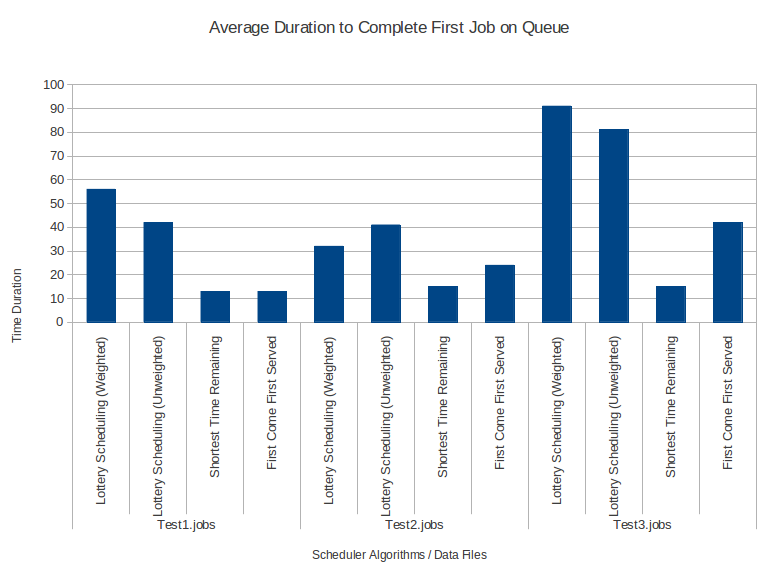
\includegraphics[scale=0.29]{graph_firstjobtime1.png}
\caption{Graph detailing the average time to complete the first job for all algorithms with various job queues.}
\end{figure}

From the graph it is clear to see that the shortest remaining time algorithm does appear to consistently process jobs with a smaller execution time first. The first come first served algorithm does also appear to process some smaller jobs first, however both lottery scheduling algorithms do appear to quite frequently processes larger jobs first. 

\subsubsection{Large Job Lengths}
The data files provided for this test contained a variety of jobs all with a different range of idle times, priorities and lengths. However as indicated by the graph above, the average time duration for first jobs processed by the shortest remaining time algorithm were significantly low. Therefore, to confirm that the results above are an accurate representation of the output of the algorithms, and not just coincidence due to the average length of jobs in the data files, a second test was run using a collection of jobs that all had significantly greater job lengths.

\begin{figure}[!htbp]
\centering
\includegraphics[scale=0.3]{graph_firstjobtime2.png}
\caption{Graph detailing the average time to complete the first job for all algorithms using a bespoke data file with large job lengths.}
\end{figure}

Figure 2 clearly shows that even with the lengths of all the jobs in the new data file being significantly higher (when comparing time duration with Figure 1) the shortest time remaining algorithm does appear to process the job with the shortest time duration first. 

\subsection{Mean Time Duration for Single Job}

The purpose of this next test was to record the average (mean) time that each scheduler took to process a single job. This would allow the average turnaround time (an element of the latency) for the algorithm to be determined. Again, similar to the first test the average mean duration times have had to be taken to accommodate the non-deterministic schedulers. 

Two different tests were conducted to investigate how the latency of the algorithms differed depending on the kind, and quantity of jobs being processed. 

The first test involved the use of the three default test data files. ``\textit{Test.jobs}" contained a small number of jobs with relatively short job lengths, ``\textit{Test2.jobs}" contained a slightly greater number of jobs, but these had a greater number of I/O blocks that prevented the jobs from being completed in a single CPU burst, and finally ``\textit{Test3.jobs}" contained a significantly greater number of jobs, some of which finished quickly, and others that did not.  

\begin{figure}[!htbp]
\centering
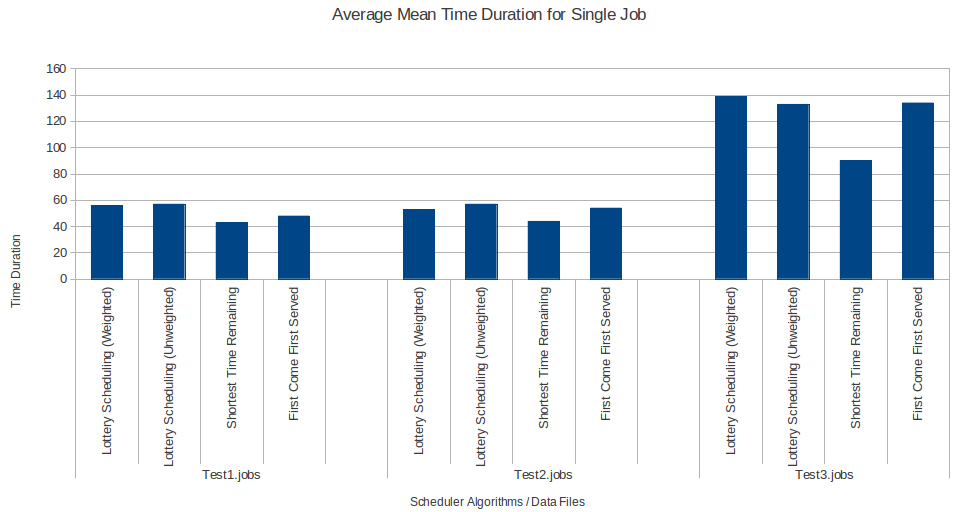
\includegraphics[scale=0.25]{graph_meantime1.png}
\caption{Graph detailing the average mean time duration to complete a single job for all algorithms using the three default data files.}
\end{figure}

In this test, the shortest remaining time algorithm does appear to consistently processes a single job faster than the other algorithms, with the other three algorithms performing similarly in all three sub-tests.

\subsubsection{Process Weighting}
The second of the two tests was designed to investigate whether the weighting of processes affected the mean time duration of the non-deterministic algorithms, and as a result two new data files were created. The first ``\textit{Test\_LongWeighted.jobs}" contained a collection of jobs that became progressively longer, the greater the priority. The second, ``\textit{Test\_ShortWeighted.jobs}" contained a number of jobs that had progressively shorter job lengths, the greater the priority.

\begin{figure}[!htbp]
\centering
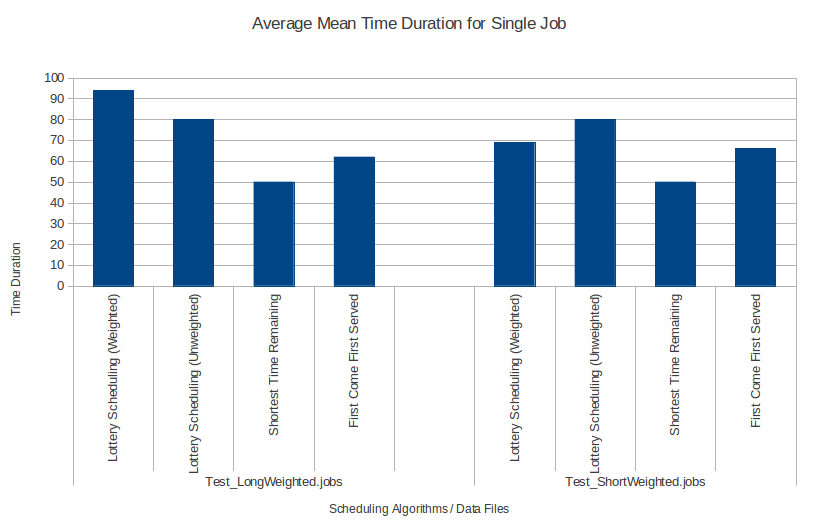
\includegraphics[scale=0.3]{graph_meantime2.png}
\caption{Graph detailing the average mean time duration to complete a single job for all algorithms using weighted jobs of varying length.}
\end{figure}

In the first sub-test the weighted version of the lottery scheduling algorithm does indeed take longer to process a single job on average that it's non-weighted counterpart. This is reflected in the second sub-test as the same algorithm this time processes a single job in a shorter duration that the non-weighted lottery scheduler. 

Both the non-weighted probabilistic algorithm, and the preemptive deterministic algorithm take the exact same average time to complete a single job in both tests. However, the non-preemptive deterministic algorithm does take slightly longer to complete in the second sub-test.

\subsection{Overall Processing Time for All Jobs}

This test aimed to investigate the total time each scheduling algorithm took to complete all the waiting processes in it's allocated job queue. This was measured by recording the total number of CPU cycles the simulator took to complete a run. 

As with the other tests, the average processing time for 5000 simulation runs was recorded as the resulting value to allow measurement of the non-deterministic algorithms.

\begin{figure}[!htbp]
\centering
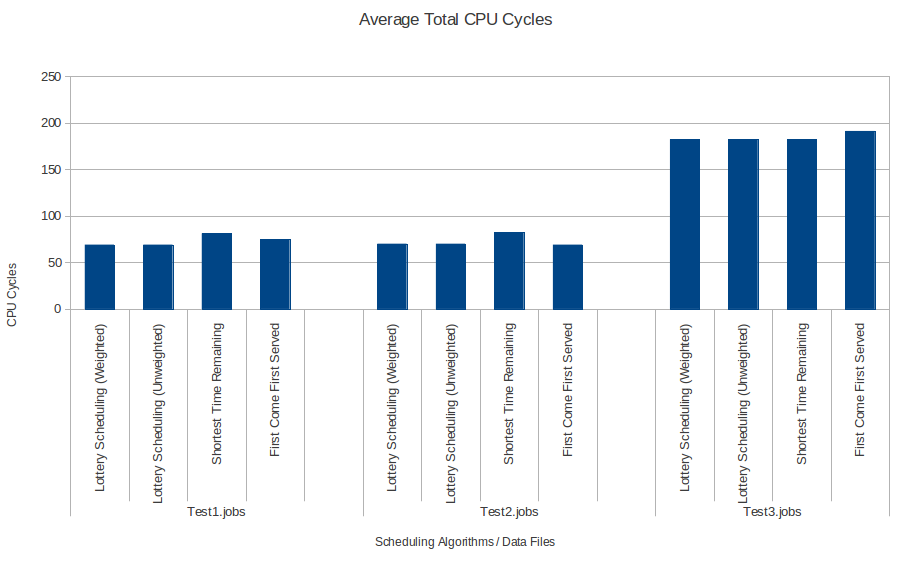
\includegraphics[scale=0.27]{graph_cpucycles1.png}
\caption{Graph detailing the average total number of CPU cycles for each algorithm when processing the three default data files.}
\end{figure} 

The test results indicate that the shortest time remaining algorithm does on average tend to take slightly longer to complete all of the waiting processes in it's job queue than the other three algorithms. 

Somewhat surprisingly, the probabilistic algorithms are faster than the deterministic algorithms to complete all of their jobs, and even more interestingly, both the weighted and non-weighted lottery schedulers take exactly the same amount of time to complete on all three sub-tests. 

\subsubsection{Cycle Blocking}

To investigate whether the blocking of CPU cycles affects the overall completion time of the algorithms, two more sub-tests were created. The first test processed a collection of jobs that all contained a high level of CPU blocks. The second test processed a collection of jobs with no CPU blocks at all.

The two tests were run and their results compared to try and identify if the halting of executing processes (e.g. for I/O processes) affected the time taken for the algorithms to complete their job queues.

\begin{figure}[H]
\centering
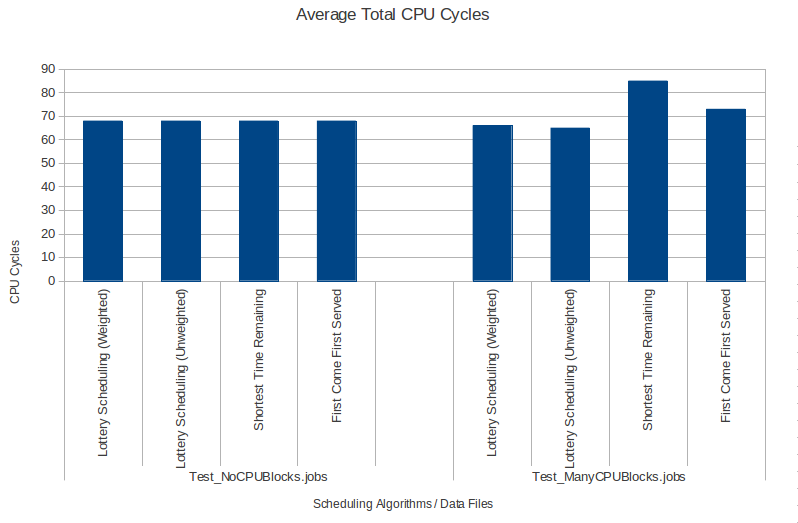
\includegraphics[scale=0.3]{graph_cpucycles2.png}
\caption{Graph detailing the average total number of CPU cycles for each algorithm when processing job queues with no CPU blocks (1) and many CPU blocks (2).}
\end{figure} 

From the graph above, it can be seen that when processing a job queue that contains no CPU blocks, all four algorithms require the exact same number of CPU cycles (68) to complete. Whereas in the second test, the results clearly indicate that the deterministic and preemptive shortest remaining time algorithm takes significantly longer to complete than the other three algorithms. 

In addition unlike all the previous tests, the non-weighted lottery scheduling algorithm processes the same collection of jobs in sub-test two slightly faster than it's weighted counterpart. 

\section{Discussion}

The results detailed above help to provide an insight into the behavior and performance of each of the four scheduling algorithms selected for this investigation. These can compared and contrasted to help identify the strengths, and weaknesses of each algorithm. 

\vfill
\subsection{Time Duration of First Job}

Both tests to identify the average duration of the first job for each of the four algorithms appears to support the prediction detailed in hypothesis one (\textbf{See Fig:1}). 

Consistently, the shortest time duration of the first job to be executed was registered from the only preemptive algorithm out of the four under testing (shortest remaining time). This is due to the fact that the behavior of the algorithm is such, that it will always choose the job with the shortest remaining execution time to run next. This means that typically once a job has been started by the algorithm, it is rare for the that job to stop executing until it is complete, as there would typically not be a high probability of a job that has yet to begin executing, having a shorter execution time than the remaining time left of the job currently in execution. If this was the case however, then the algorithm would then indeed switch to that shorter job. 

The results obtained for the first come first served algorithm initially appear to indicate that the length of time required for the first job to complete may correlate in someway to the number of jobs in the queue, or the length of jobs. While this is partially true,  further testing (\textbf{See Fig:2}) reveals that the results for the algorithm are solely determined by the length of the original job located in the first position of the queue when the tests are run. In other words, as the algorithm is non-preemptive, no changes are made at all to the original queue loaded in from the test data files. This means that the job at the front of the queue will always be processed first, regardless of the length, and so simply re-arranging the order of the jobs in the data files could potentially change this value. This however, should not be the case with the shortest remaining time/lottery scheduling algorithms.

The priority of jobs (utilised by the weighted lottery scheduling algorithm) could potentially affect the time duration (as higher priority jobs have a greater chance of being selected next) however there is no definite guarantee that a job with a higher priority would indeed be picked, and if it was picked, no guarantee that particular job would have a higher or shorter length than any other job in the queue.

\subsection{Mean Time Duration for Single Job}

From analysing the results obtained for mean time duration of a single job (\textbf{See Fig:3 \& Fig:4}), it would appear that utilising a preemptive, deterministic algorithm over a non-preemptive/non-deterministic algorithm does indeed reduce the average time taken to complete a single job as detailed in hypothesis three. 

A possible reason for this is the fact that as jobs are selected by remaining execution time from smallest to largest, jobs once started are unlikely to be halted again before they are completed (other than for events such as CPU blocks). This will therefore result in the overall average time to complete that particular job being reduced. 

However, the results obtained cannot be assumed to be entirely conclusive,  as the value used to represent the time duration for a single job is a mean average of the total duration of all the jobs, and so some jobs will inevitably take longer to complete than others if they have a longer length, and/or are interrupted by another (higher priority) process.

Interestingly and somewhat surprisingly, the results obtained for the first come first served algorithm appear to contradict the reasoning made for the significantly shorter mean time duration recorded for shortest remaining time algorithm. In all the tests conducted (\textbf{detailed in Fig:3 \& Fig:4}) the first come first served algorithm takes, on average, significantly longer to complete a single job than that of the shortest time remaining algorithm. According to the reasoning discussed above about the results of the STR algorithm, this should not be the case, as both algorithms (\textbf{normally} in the case of STR, and \textbf{always} in the case of FCFS) process a job until completion before selecting the next job, and so therefore according to the logic of the reasoning discussed above, should have equal (or very similar to account for abnormalities) mean duration times for a single job. However clearly, this is not the case. 

The most likely reason for this unexpected difference in results is the fact that a sheer coincidence in the ordering of the jobs within the data files, is causing the first come first served algorithm to perform a larger number of context switches as it processes the jobs with a greater frequency of CPU blocks one after another. This difference in ordering could affect the \textit{average} time duration significantly enough to cause the unexpected results that are being experienced. 

The non-deterministic lottery scheduling algorithms produced fairly consistent results across the first three tests detailed in \textbf{Fig:3}. In the first two tests the weighted version of the lottery scheduling algorithm performed slightly better than it's non-weighted counterpart. After an analysis of the two data files, it would appear that this was the case because the jobs with a higher priority (and so greater chance of being selected) had less CPU blocks than other jobs, and so could be completed in less time. Similar reasoning is used to explain the change in performance between the two algorithms within the third test. The more heavily weighted jobs in the third data file have a greater number of CPU blocks than the less priority jobs, resulting in the weighted version of the algorithm performing slightly slower. 

In an attempt to investigate the extent to which the weighting of jobs affects the performance between the two lottery scheduling algorithms, a further two tests were run (\textbf{See Fig:4}). The results of the tests came back as expected, with the weighted algorithm performing slower in the fourth test (due to the higher priority jobs having a longer job length), and performing better in the final test due to the higher priority jobs having shorter job lengths.

Comparing the two lottery scheduling algorithms against to the other two algorithms being tested, it is apparent that the non-deterministic algorithms have consistently slower mean time durations for completing a single job. This is most likely to be because of the random nature of both algorithms, potentiality resulting in jobs with a greater number of CPU blocks being chosen more consistently than other algorithms that specifically decide which job to run next based on their information.

\vfill 

\subsection{Overall Processing Time for All Jobs}

The collection of results produced by these series of tests appears to disprove the original hypothesis predicting that a weighted probabilistic algorithm would take longer to complete all jobs than the non-weighted version of the same algorithm. 

Throughout all of the first three sub-tests (\textbf{See Fig:5}) both the weighted, and non-weighted lottery scheduling algorithms took the exact same number of CPU cycles to complete their job queues. This was surprising as it was initially predicted that because the weighted lottery scheduling algorithm had to re-allocate a set number of tickets to every waiting job (based on it's priority) every time a new job was selected, this would result in the non-weighted version (which did not have to process any allocation of new tickets) running faster overall. 

However, in the final sub-test performed (\textbf{See Fig:6}) it does appear that the weighted lottery scheduling algorithm does take slightly longer to process all the jobs, and so is the first sub-test to support the original hypothesis. This however was expected, as in the same test the jobs with a higher weighting (and therefore greater chance of being selected next) all had progressively larger and more frequent CPU blocks. 

The preemptive shortest remaining time algorithm took the highest number of CPU cycles to complete in three of the five sub-tests that were carried out. The most likely reason for this is because of the additional cycles that are required every time a new job is added, or an existing job is returned to sort the job queue based on the shortest remaining execution time. Following on from this, the results of the fourth sub-test (\textbf{See Fig:6}) indicate that when no CPU blocks are processed, all four algorithms take an exactly equal number of CPU cycles to complete their job queues. This further supports the idea that due to the fact that jobs are being returned to the job queue (because of CPU blocks), preemptive algorithms like SRT that have to perform additional processing every time a new job is added or returned will take an increased number of CPU cycles to complete all of their allocated jobs.  

Similarly, the overall processing time for the first come first served algorithm appears to depend on the order in which it processes the jobs, and the length/frequency of CPU blocks within those jobs. This idea is again supported by the results of the fourth sub-test (\textbf{See Fig:6}) showing that all four algorithms take exactly the same overall processing time when no CPU blocks are apparent in the data file. The outcome of these results would normally be expected of a non-preemptive, deterministic algorithm such as FCFS, as it would simply process jobs in the original order that they arrive in the queue with no additional sorting/processing, and so hence explaining why the FCFS algorithm on average, takes less CPU cycles than SRT to complete.

\section{Conclusion} 

\subsection{Time Duration of First Job}

From the analysis of the results, it has been identified that a preemptive, deterministic algorithm such as shortest time remaining does indeed process jobs with the shortest remaining execution time first, and thus supports the hypothesis explaining that due to the preemptive behavior of such as algorithm, jobs with a short execution time will be selected and processed as a priority. 

\subsection{Mean Time Duration for Single Job}

It can be concluded from the results that the use of preemptive algorithms can help to reduce the mean time taken to complete a single job, as predicted in the second hypothesis. 

It is worth noting however that this can be heavily affected by the length and frequency of CPU blocks apparent within the waiting processes at any particular moment in time. 

\subsection{Overall Processing Time for All Jobs}

Contradicting the original prediction made in the third and final hypothesis, there is no concrete evidence to suggest that the extra processing required for a weighted non-deterministic algorithm causes it to be slower at processing all of it's allocated jobs that the non-weighted equivalent algorithm, and instead appears to depend more on the frequency and length of CPU blocks within the higher priority jobs that have a larger weighting. 

In addition, it can be concluded that the non-deterministic scheduling algorithms tend to be consistently faster at processing job queues as a whole, than the deterministic algorithms (both preemptive and non-preemptive) tested.

%\end{document}  % This is where a 'short' article might terminate

\section{Executive Summary}

This purpose of this investigation was to compare and contrast the performance of scheduling algorithms when supplied with varying collections of jobs. These algorithms were implemented into an existing simulator application developed in Java, and tested using a variety of data files. The major findings of this investigation reveal that in general, preemptive algorithms can provide a higher level of throughput, while non-deterministic algorithms can consistently process collections of jobs as a whole in less time, and so provide better latency. 

%
% The following two commands are all you need in the
% initial runs of your .tex file to
% produce the bibliography for the citations in your paper.
\bibliographystyle{abbrv}
\bibliography{sigproc}  % sigproc.bib is the name of the Bibliography in this case
% You must have a proper ".bib" file
%  and remember to run:
% latex bibtex latex latex
% to resolve all references
%
% ACM needs 'a single self-contained file'!
%
%APPENDICES are optional
%\balancecolumns
\appendix
%Appendix A
% This next section command marks the start of
% Appendix B, and does not continue the present hierarchy
\textbf{Appendix 1}: Implementation Design\\
\textbf{Appendix 2}: Algorithms System Testing

\begin{thebibliography}{1}

 \bibitem{notes} R.Shipman {\em ``CS21120 Assignment 2 - Scheduling"} 2013: Aberystwyth University, Aberystwyth.
 
  \bibitem{notes} {\em ``Scheduling (computing)"} http://en.wikipedia.org/wiki/Scheduling\_(computing) Wikipedia, Wikimedia Foundation Inc.
  
  \bibitem{notes} {\em ``Shortest remaining time"} http://cs.kent.edu/farrell/osf03/oldnotes/L18.pdf Kent University, Ohio
  
   \bibitem{notes} {\em ``1998 ACM Computing Classification System"} http://www.acm.org/about/class/ccs98-html Associateion for Computing Machinery.
   
    \bibitem{notes} {\em ``Writing Scientific Papers"} http://colby.edu/biology/Bl17x/writing\_papers/ Colby University, Waterville ME.
  
 \end{thebibliography}
\end{document}
